\documentclass[../main.tex]{subfiles}

\begin{document}

\section{Change Detection Algorithms}

Change detection first came about as a quality control measure in manufacturing, and methods within this domain are generally referred to as \emph{control charts}. Since the inception of approaches such as CUSUM \cite{Page1954} that provide the possibility for on-line evaluation of continuous data streams, change detection has grown as a field. With applications such as epidemic detection, online reputation management and infrastructure error detection, change detection is hugely useful both as an academic problem and in production systems of myriad application.

As the name suggests, change point detection methods are methods by which some \emph{change} can be detected in some data, be it a change in mean, variance or some other measure. Change point detection also encompasses the field of anomaly or outlier detection.

This thesis work utilises three different change point detection methods, discussed forthwith.

\subsection{Pruned Exact Linear Time}

Pruned Exact Linear Time (\emph{PELT}) is a modern change point detection method proposed by \citeauthor{Killick2011a} in \citetitle{Killick2011a}, in 2012 \cite{Killick2011a}.

PELT is an \emph{exact} method of computing change points, based on segmentation of data streams, in the same manner as Segment Neighbourhood and Binary Segmentation, the two other algorithms being utilised in this work. PELT is a modification of the \emph{Optimal Partitioning} method proposed by \citeauthor{Jackson2003} in 2003 \cite{Jackson2003}.

Jackson's method has a computational cost of $O(n^2)$, while Killick's PELT method improves on this with a computational complexity of $O(n)$ \cite{Killick2011a}. PELT achieves this by introducing a `pruning' step in the algorithm (as the name suggests) in which as the algorithm iterates, it removes any values of $\tau$ (see Algorithm \autoref{alg:pelt} for definition) that could not possibly be a minima of the operation in line 2 of Algorithm \autoref{alg:pelt}.

The PELT method works similarly to Segment Neighbourhood \cite{Auger1989} and Binary Segmentation \cite{Jackson2003, Yao1984} approaches (described in the following sections), in that it attempts to fit a model of segmentation of a given data set, minimising the cost of the segmentation to achieve an optimal distribution of segments and therefore change points.

Algorithm \autoref{alg:pelt} describes a pseudocode implementation of the PELT algorithm, as described by \citeauthor{Eckley2011} in \citetitle{Eckley2011} \cite{Eckley2011}\newline

\begin{algorithm}[H]
    \label{alg:pelt}
    \caption{PELT Method for change point detection}
    \DontPrintSemicolon
    \SetKwInOut{Initialise}{Initialise}
    \KwIn{A set of data of the form, $(y_1, y_2, \ldots,y_n)$ where $y_i \in \mathbb{R}$.\newline
        A measure of fit $C(.)$ dependent on the data.\newline
        A penalty constant $\beta$ which does not depend on the number or location of change points.\newline
        A constant $K$ that satisfies $C(y_{(t+1):s}) + C(y_{(s+1):T}) + K \leq C(y_{t+1):T})$\newline}
    \Initialise{Let $n$ = length of data and set $F(0) = -\beta$, $cp(0) = NULL$\newline}
    \For{$\tau* = 1,\ldots,n$}{
        Calculate $F(\tau*) = min_{\tau \in R_{\tau*}} \lbrack F(\tau) + C(y_{\tau+1:\tau*}) + \beta \rbrack$\;
        Let $\tau^1 = arg \Big\{ min_{\tau \in R_{\tau*}} \lbrack F(\tau) + C(y_{(\tau+1):\tau*}) + \beta \rbrack \Big\}$\;
        Set $cp(\tau*) = \lbrack cp(\tau^1), \tau^1 \rbrack$\;
        Set $R_{\tau^* + 1} = \{\tau \in R_{\tau^*} \cup \{\tau^*\} : F(\tau) + C(y_{\tau+1:\tau^*}) + K \leq F(\tau^*)\}$\;
    }\bigskip
    \KwOut{the change points recorded in $cp(n)$}
\end{algorithm}

\subsection{Segment Neighbourhoods}

Proposed by Auger and Lawrence in 1989 \cite{Auger1989}, Segment Neighbourhood (\emph{SegNeigh}) is an example of an exact segmentation algorithm for the detection of change points in data. SegNeigh utilises dynamic programming to search the segmentation space (defined as the maximum number of change points in a given data stream) and then compute the cost function for every possible segmentation of the data. In this way, the location and number of change points can be computed exactly by taking the segmentation that returns the lowest cost function result.

Segment Neighbourhoods has a computational complexity of $O(n^2)$, significantly higher than that of PELT or Binary Segmentation. However, this additional cost in complexity is offset by improved performance when compared to Binary Segmentation, as shown by \citeauthor{Braun2000} in \citetitle{Braun2000} \cite{Braun2000}.

Algorithm \autoref{alg:segneigh} describes a pseudocode implementation of the SegNeigh algorithm, as described by \citeauthor{Eckley2011} in \citetitle{Eckley2011} \cite{Eckley2011}\newline

\begin{algorithm}[H]
\label{alg:segneigh}
    \caption{Generic Segment Neighbourhoods method for change point detection}
    \DontPrintSemicolon
    \SetKwInOut{Initialise}{Initialise}
    \SetKwInOut{Input}{Input}
    \SetKwInOut{Output}{Output}
    \KwIn{A set of data of the form, $(y_1, y_2, \dots, y_n)$\newline
        A measure of fit $R(.)$ dependent on the data which needs to be minimised.\newline
        An integer, $M-1$ specifying the maximum number of change points to find.}
    \Initialise{Let $n$ = length of data.\newline
        Calculate $q^1_{i,j} = R(y_{i:j})$ for all $i, j \in \lbrack 1,n \rbrack$ such that $i < j$.\newline}
        
    \For{$m = 2, \ldots ,M$}{
        \For{$j \in \{1,2,\ldots , n\}$}{
            Calculate $q^m_{1,j} = min_{v \in \lbrack 1,j \rbrack }(q^{m-1}_{1,v} + q^1_{v + 1, j})$\;
        }
        Set $\tau_{m, 1}$ to be the $v$ that minimises $(q^{m-1}_{1,v} + q^1_{v + 1, n})$\;
        \For{$i \in \{ 2, 3, \ldots , M \}$}{
            Let $\tau_{m,i}$ to be the $v$ that minimises $(q^{m-i-1}_{1,v} + q^1_{v + 1, cp_{m,i-1}})$\;
        }
        
    }\bigskip
        
    \KwOut{For $m = 1, \ldots , M$: the total measure of fit, $q^m_{1,n}$ for $m-1$ change points and the location of the change points for that fit, $\tau_{m,1:m}$.}
\end{algorithm}

\subsection{Binary Segmentation}

Binary Segmentation \cite{Jackson2003, Yao1984} (\emph{BinSeg}) is a popular method for change point detection, widely utilised in the field. Binary segmentation is a method that recursively applies a single change point detection method. On the first iteration, if a change point is detected, the data is split around that change point (resulting in two data sets) and the change point method is run again on the two resulting data sets. This process is repeated such that many data set segments are created, and runs until no further change points are detected.

BinSeg is an \emph{approximate} change point detection approach, and returns estimated change point locations - unlike PELT and SegNeigh - which return exact change point locations. It has the same computational cost as PELT, $O(n)$.

Algorithm \autoref{alg:binseg} describes a pseudocode implementation of the BinSeg algorithm, as described by \citeauthor{Eckley2011} in \citetitle{Eckley2011} \cite{Eckley2011}\newline

\begin{algorithm}[H]
    \label{alg:binseg}
    \caption{Generic Binary Segmentation method for change point detection}
    \DontPrintSemicolon
    \SetKwInOut{Initialise}{Initialise}
    \SetKwInOut{Input}{Input}
    \SetKwInOut{Output}{Output}
    \KwIn{A set of data of the form, $(y_1, y_2, \dots, y_n)$\newline
    A test statistic $\Lambda(.)$ dependent on the data\newline
    An estimator of change point position $\hat{\tau}(.)$\newline
    A rejection threshold $C$.\newline}
    \Initialise{Let $\mathcal{C} =\emptyset$, and $\mathcal{S} = \{ \lbrack 1,n \rbrack \}$\newline}
    \While{$\mathcal{S} \neq \emptyset$}{
        Choose an element of $\mathcal{S}$, denote element as $\lbrack s,t \rbrack$\;
        \If{$\Lambda(y_{s:t}) < C$}{
            remove $\lbrack s,t \rbrack$ from $S$\;
        }
        \If{$\Lambda(y_{s:t}) \geq C$}{
        
            remove $\lbrack s, t \rbrack$ from $\mathcal{S}$\;
            calculate $r = \hat{\tau}(y_{s:t}) + s - 1$, and add $r$ to $\mathcal{C}$\;
            
            \If{$r \neq s$}{
                add $\lbrack s, r \rbrack$ to $\mathcal{S}$\;
            }
            
            \If{$r \neq t - 1$}{
                add $\lbrack r + 1, t \rbrack$ to $\mathcal{S}$\;
            }
        }
    }\bigskip
    \KwOut{the set of change points recorded in $\mathcal{C}$}
\end{algorithm}

\section{Algorithm Configuration}

Change detection is an \emph{unbounded} problem. Left without some system of constraint, the algorithm could theoretically run to infinity. Indeed, experiments carried out at the beginning of this research showed that one of the algorithms utilised in this research, PELT, when left unbounded, will detect every data point in the time-series as a change point. This result is \textit{technically} correct, but not useful for our purposes. For this reason, the algorithms implement a penalty system, allowing for an optimal number of change points to be detected.

\subsection{Penalty Scores}

Penalty scores operate as a mechanism for optimising an unbounded problem such as the one being addressed here. Publications on the subject (such as \citetitle{Haynes2014} by \citeauthor{Haynes2014} \cite{Haynes2014}) define the problem as follows: Given time series data points $y_1,\ldots,y_n$, the series will contain $m$ change points such that their locations $\tau_{1:m} = (\tau_1,\ldots,\tau_m)$, where $\{\tau_i \in \mathbb{Z} \mid 1 \leqslant \tau_i \leqslant n-1\}$. $\tau_0$ is assumed to be 0, and $\tau_{m+1}$ is assumed to be $n$. In this way we can state that a given change detection algorithm will split the time series into $m + 1$ segments such that segment $i$ contains the points $y_{(\tau_{i-1}+1):\tau_i} = (y_{\tau_{i-1} + 1},\dots,y_{\tau_i})$. A \emph{cost function} for a segmentation of the data set $y_s$ can be defined as $C = (y_{s+1:t})$. This cost function defines a cost for a given segmentation containing points $y_{s+1:t}$. To illustrate, the cost function $C$, in the context of binary classification, returns a value that increases for an `incorrect' classification and decreases for a `correct' classification. More intuitively, $C$ can be defined as a value that decreases when a change point is introduced into a segmentation being passed as an argument to $C$.

At this point it can be stated that the \emph{constrained minimisation problem} is as follows:

\begin{equation}
\label{unbounded}
    Q_m(y_{1:n}) = \min_{\tau_{1:m}} \Bigg\{ \sum^{m+1}_{i=1}[C(y_{(\tau_{i - 1} + 1):\tau_i})] \Bigg\}
\end{equation}

\autoref{unbounded} is an equation showing the optimisation problem that change point detection presents. If the equation is taken intuitively, it shows that for a dataset with a \emph{known} number of change points, the segmentation of the data around the change points can be effectively estimated by obtaining the segmentation that returns the minimum total cost based on the sum of cost function $C$.

However, the problem being solved by many change detection algorithms involves an unknown number of change points, at unknown locations. In this case we can estimate the following to obtain the number and location of the change points:

\begin{equation}
\label{eqn:penalty}
    \min_{m} \big\{ Q_m(y_{1:n}) + f(m) \big\}
\end{equation}

\autoref{eqn:penalty} includes a \emph{penalty function} $f(m)$ that increases proportionally with the number of change points $m$. Essentially, as the segmentation calculated as $Q_m$ increases in size, so does the result of the penalty function $f(m)$. These two elements are at-odds with each other, presenting a problem that requires optimisation to correctly estimate the number and location of change points in the data set $y_s$. If $f(m)$ increases in a linear fashion with $m$, we can define a \emph{penalised minimisation problem} in the following manner:

\begin{equation}
\label{bounded}
    Q_m(y_{1:n}, \beta) = \min_{m,\tau_{1:m}} \Bigg\{ \sum^{m+1}_{i=1}[C(y_{(\tau_{i - 1} + 1):\tau_i}) + \beta] \Bigg\}
\end{equation}

In this equation, $\beta$ is the penalty function defined previously as $f(m)$.

There are a number of established approaches to calculating penalty values for unbounded problems, chiefly among which are Schwarz Information Criterion (SIC)/Bayesian Information Criterion (BIC) \cite{Schwarz1978}, Akaike Information Criterion (AIC) \cite{Akaike1974} and Hannan-Quinn \cite{Journal2009}. Of these approaches, it is necessary to experiment to find the scheme that produces the `correct' number of change points for a given dataset. The penalty schemes are defined as follows:

\begin{align}
    \text{SIC} &= \ln(n) k - 2 \ln(\hat{L})\\
    \text{AIC} &= 2k - 2 \ln(\hat{L})\\
    \text{HQC} &= -2L_{max} + 2k \ln(\ln(n))
\end{align}

Where $n$ is the total number of observations, $k$ is the number of \emph{free parameters}\footnote{variables that are unable to be predicted by a given model} and $\hat{L}$ is the maximum value of a likelihood function.

The penalty function returns a value which is represented by $\beta$ in \autoref{bounded}, which then limits the number of possible segmentations returned by $Q$. In this way, varying the penalty function $\beta$ can alter the results given by a change detection algorithm by increasing or decreasing the number of change points detected.

The \texttt{changepoint} package requires the provision of a penalty function for each algorithm, which has been chosen as `SIC' for this research. This decision is based upon advice published in \cite{Eckley2011}, in which it is stated that AIC (while popular in the field of change point detection as a penalty term) tends to asymptotically overestimate $k$.

While the selection of an optimal penalty term for a given data set and change point detection algorithm is an open research question in itself. There exists a method, \emph{Changepoints for a Range of Penalties} (CROPS) \cite{Haynes2014}, in which a change detection algorithm (PELT, in this case) is repeatedly executed in such a fashion that allows for the plotting of the number change points detected against the penalty value used. When conducting analysis against a single, static data source (offline analysis), this method can be useful for ensuring optimal penalty term selection.

\begin{figure}[h]
\centering
    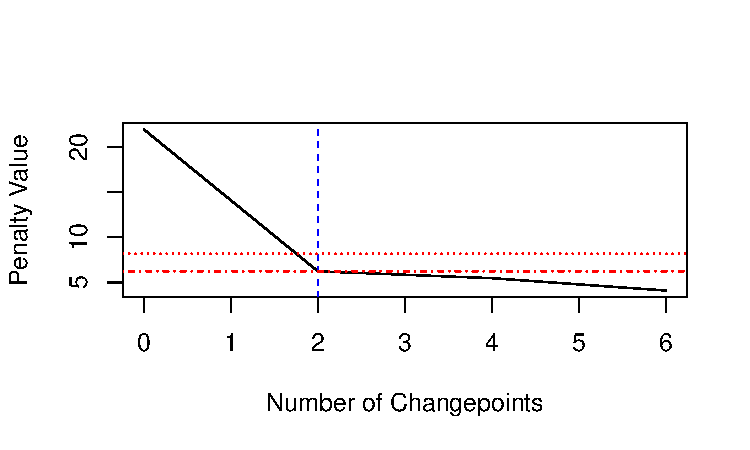
\includegraphics[width=0.5\textwidth]{figures/CROPS2}
    \caption{CROPS Algorithm Output}
    \label{fig:CROPS}
\end{figure}

\autoref{fig:CROPS} shows an example of the output of the CROPS algorithm, when executed against the `Rabobank' data set used in the real-world data analysis. To read this output, the optimal penalty value should be chosen such that the plot at that point has begun to level off, showing a fast increase in the number of change points for penalty values lower than this. This example shows an optimal penalty value of about 6 (backed up by the algorithm output of a penalty value of 6.21 for 2 change points - signified by the dash-dot red line on the plot). The penalty value for the same data set computed with SIC is 8.16 (signified by the dotted red line on the plot), which also results in a total of two change points being detected. Because the PELT algorithm has a computational complexity of $O(n)$, if it is necessary to carry out an analysis such as this for a static data set, it would be easy to do so.

However, the usefulness of such a method for application to streaming (online) data sets is questionable.


\subsection{Distribution Assumptions}

It is also important to note that many change point detection methods make an assumption about the underlying distribution of the data being analysed. This distribution can be, for example, a normal distribution, poisson distribution or a gamma distribution. The selection of this distribution can have an effect on the ability of a given algorithm to detect change points.

To limit the scope of this research, an assumption is made that all of the data being analysed follows a normal distribution, to allow for a `like for like' comparison of results. It is possible for some algorithms to use a CUSUM test statistic that makes no assumptions about data distribution, but this is not supported by all of the methods implemented in \texttt{changepoint}. It is also possible to specify a poisson or gamma distribution when utilising the mean/variance test statistic, but this has not been done in this research, again, in order to ensure a `like for like' comparison of approaches.

\section{Evaluation Measures}

As briefly discussed in the introduction to this thesis, there are a number of pre-existing approaches for the evaluation of change detection methods. Here, the measures being evaluated are briefly explained:

\subsection{F1 Score}

This measure is utilised for testing accuracy in problems of binary classification. It considers two different measures, \emph{precision} and \emph{recall}, and takes a harmonic mean of the two measures to compute the final score. This measure is used in research by \citeauthor{Qahtan2015} \cite{Qahtan2015}, \citeauthor{Buntain2014} \cite{Buntain2014}, and \citeauthor{Pelecanos2010} \cite{Pelecanos2010} (among others) for the purposes of evaluating change point detection methods.
	
	To calculate Precision and Recall, a \emph{confusion matrix} such as that in \autoref{confusionmatrix} is first constructed to provide values for the total number of true positives, false negatives, false positives and true negatives:
	
	\begin{figure}[H]
	\begin{center}
	    \begin{tikzpicture}[box/.style={draw,rectangle,minimum size=2cm,text width=1.5cm,align=center}]
            \matrix (conmat) [row sep=.1cm,column sep=.1cm] {
            \node (tpos) [box,
               label=left:\( \mathbf{p'} \),
                label=above:\( \mathbf{p} \),
            ] {True \\ Positive};
            &
            \node (fneg) [box,
                label=above:\textbf{n},
                label=above right:\textbf{Totals},
                label=right:\( \mathrm{P}' \)] {False \\ Negative};
            \\
            \node (fpos) [box,
                label=left:\( \mathbf{n'} \),
                label=below left:\textbf{Totals},
                label=below:P] {False \\ Positive};
            &
            \node (tneg) [box,
                label=right:\( \mathrm{N}' \),
                label=below:N] {True \\ Negative};
            \\
            };
    
            \node [rotate=90,left=.05cm of conmat,anchor=center,text width=1.5cm,align=center] {
                \textbf{Actual Value}
            };
            \node [above=.05cm of conmat] {\textbf{Prediction Outcome}};
            
        \end{tikzpicture}
        \caption{Confusion Matrix Example}
        \label{confusionmatrix}
        \end{center}
	\end{figure}
		
	Precision and Recall were proposed by \citeauthor{Kent1955}, in \citetitle{Kent1955}, for the purposes of scoring the effectiveness of information retrieval methods \cite{Kent1955}.
		
	$Recall$ is computed as the number of correct positive results, divided by the number of positive results that should have been detected. $Precision$ is computed as the number of correct positive results divided by the number of all possible positive results:
	
	\begin{eqnarray}
	    Precision = \frac{TP}{TP + FP}\\
	    Recall = \frac{TP}{TP + FN}
	\end{eqnarray}
		
	The F1 score calculation (the harmonic mean of both recall and precision) can be described in general terms as follows \cite{VanRijsbergen1979}:

	\begin{equation}
		F_1 = 2 \cdot \frac{1}{\frac{1}{recall} + \frac{1}{precision}} = 2 \cdot \frac{precision \cdot recall}{precision+recall}
		\label{equ:F1}
	\end{equation}

    The F1 score was first proposed by \citeauthor{VanRijsbergen1979} in his seminal work, \citetitle{VanRijsbergen1979}.

	As the F1 score is a binary classification measure, it can only be used to test the precision of an algorithm in a single domain, that is, was the change detected or not. Precision, Recall and F1 Score all provide a score $s$ such that $ \{s\in\mathbb{R} \mid 0\leq s \leq 1\} $.

\subsection{Rand Index}

This measure is for computing the similarity between two clusters of data points. It is used for calculating the overall accuracy of a given clustering approach, when compared against a set of ground truth clusters. It was first proposed by \citeauthor{Rand1971} in \citetitle{Rand1971} \cite{Rand1971}. It was used by \citeauthor{Matteson2012} in \citetitle{Matteson2012} for the purposes of evaluating change point detection approaches \cite{Matteson2012}. The Rand Index is defined as:

	\begin{equation}
		R = \frac{a+b}{a+b+c+d}
	\end{equation}
	
	Given a set of data points $S$, partitioned through two different methods, which shall be referred to as $X$ and $Y$, the following can be defined:
	
	\begin{itemize}
		\item $a$ = total number of pairs that were partitioned into the \emph{same} subset by both $X$ and $Y$
		\item $b$ = total number of pairs that were partitioned into \emph{different} subsets by both $X$ and $Y$
		\item $c$ = total number of pairs that were partitioned into the \emph{same} subset by $X$ and into a different subset by $Y$
		\item $d$ = total number of pairs that were partitioned into the \emph{same} subset by $Y$ and into a different subset by $X$
	\end{itemize}
	
	Intuitively, it can be stated that $a+b$ is the total number of agreements between methods $X$ and $Y$, while $c+d$ is the total number of disagreements. This calculation will return $0$ for completely different clusters and $1$ for identical clusters. The Rand Index provides a score $s$ such that $ \{s\in\mathbb{R} \mid 0\leq s \leq 1\} $
	
\subsection{Adjusted Rand Index}
	
Similar to the Rand Index, but adjusted to take into account the random chance of pairs being assigned to the same cluster by both approaches being compared. While the Rand Index is suited for comparing a segmentation method against a known-good \emph{oracle} method, the adjusted index is also suited to comparing two differing approaches \cite{Matteson2012}. It was first proposed by \citeauthor{Hubert1985} in \citetitle{Hubert1985} \cite{Hubert1985}. It was utilised as a similarity measure for computed clusters created by segmentation of data sets in \cite{Matteson2012}. It is defined as:
	
	\begin{equation}
	    R_{adjusted} = \frac{R - R_{expected}}{R_{max} - R_{expected}}
	\end{equation}
	
	where $R_{expected}$ is defined as the expected Rand Index score for two completely random classifications of the given data \cite{Matteson2012} and $R_{max}$ is defined as the maximum Rand Index value - generally $1$.
	
	The Adjusted Rand Index provides a score $s$ such that $ \{s\in\mathbb{R} \mid -1\leq s \leq 1\} $. This is different to the score returned by the `basic' Rand Index, in that it is possible for a negative value to be returned.
		
\subsection{BCubed}
		
BCubed is similar to the Adjusted Rand Index, in that it is adjusted to be appropriate for all constraints in a clustering problem. It was developed by Bagga and Baldwin in 1998 \cite{Bagga1998}.

This measure was not found to be in use for the purposes of evaluating change point detection methods, but it was particularly interesting to investigate based on \citeauthor{Matteson2012}'s use of clustering metrics \cite{Matteson2012} for this purpose. It was decided that this measure would be included as an additional well-known clustering measure, to investigate whether it would perform any better than the established Rand and Adjusted Rand indices.
	
	BCubed operates in a similar way to the F1 binary classification metric, in that it computes precision and recall values, before calculating a harmonic mean of the two metrics. BCubed also makes use of an additional \emph{correctness} function defined as follows, where $e$ and $e'$ are equivalent elements in a ground truth and computed clustering respectively, $L$ is a computed label and $C$ is a ground truth category:
	
	\begin{equation}
	\label{eqn:correctness}
	    \text{Correctness}(e,e') = 
	    \begin{cases}
	        1 & \text{iff $L(e) = L(e') \leftrightarrow C(e) = C(e')$}\\
	        0 & \text{otherwise}
	    \end{cases}
	\end{equation}
	
	\autoref{eqn:correctness} can be stated intuitively as returning $1$ if and only if both the ground truth and computed clusterings place the element $e$ into the same cluster, returning $0$ in all other cases.
	
	Precision and Recall can then be calculated as follows:
	
    \begin{align}
    \label{eqn:bcubed-precision}
        \text{Precision} &= Avg_e [Avg_{e' . C(e) = C(e')}[Correctness(e,e')]]\\
        \label{eqn:bcubed-recall}
        \text{Recall} &= Avg_e [Avg_{e' . L(e) = L(e')}[Correctness(e,e')]]
    \end{align}

To obtain the F score, a harmonic mean of Precision and Recall is taken in the same manner as the F1 score for binary classification:

\begin{equation}
    F_{bc} = 2 \cdot \frac{1}{\frac{1}{Recall_{bc}} + \frac{1}{Precision_{bc}}}
\end{equation}

The BCubed F-Score provides a score $s$ such that $ \{s\in\mathbb{R} \mid 0\leq s \leq 1\} $, much like the Rand Index and F1 score for binary classification.

\end{document}